\documentclass[border=5mm]{standalone}
\usepackage{tikz}
\usepackage{tikz-qtree}

\begin{document}
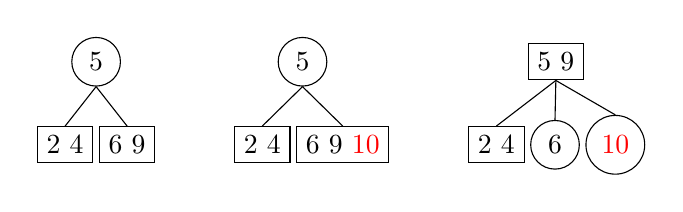
\begin{tikzpicture}[every tree node/.style={align=center}]
    \matrix[row sep=1cm, column sep=1cm] {
    \Tree
    [.\node[draw, circle](root1){5};
    [.\node[draw, rectangle]{2 4}; ]
    [.\node[draw, rectangle]{6 9}; ]
    ];
    &
    \Tree
    [.\node[draw, circle](root2){5};
    [.\node[draw, rectangle]{2 4}; ]
    [.\node[draw, rectangle]{6 9 \textcolor{red}{10}};]
    ];
    &
    \Tree
    [.\node[draw, rectangle](root2){5 9};
    [.\node[draw, rectangle]{2 4}; ]
    [.\node[draw, circle]{6}; ]
    [.\node[draw, circle]{\textcolor{red}{10}}; ]
    ]; \\
    };
\end{tikzpicture}
\end{document}
